\section{Network Designs for Disaggregation}
\label{sec:existing}

Our evaluation so far has ignored the impact of queueing delay on end-to-end latency and hence application performance. We remedy the omission in this section.
The challenge is that queueing delay is a function of the overall design of the network, including: the input traffic workload, the network topology and routing, and the end-to-end transport protocol. Our evaluation focuses on existing proposals for transport protocols, with standard assumptions about the datacenter topology and routing (described below). However, the input traffic workload in \dis will be very different from that in a server-centric datacenter and, to our knowledge, no models exist that characterize traffic in a \dis. 

We thus start by devising a methodology that extends our experimental setup to generate an application-driven input traffic workload (\S\ref{ssec:ssmethod-traffic}), then describe how we use this traffic model to evaluate the impact of queueing delay (\S\ref{ssec:ssmethod}). Finally, we present our results on: (i) how existing transport designs perform under \dis traffic workloads (\S\ref{ssec:nlp}), and (ii) how existing transport designs impact end-to-end application performance (\S\ref{ssec:alp}). To our knowledge, our results represent the first evaluation of transport protocols for \dis. %\sr{true?} \rc{PG:not true. R2C2 has that}




%In this section, we explore whether existing network designs can meet the requirements identified in \S\ref{sec:requirements}. 
%We start by describing our methodology (\S\ref{ssec:ssmethod}), then evaluate the network-level performance of a suite of network designs for \dis traffic workloads (\S\ref{ssec:nlp}), and finally evaluate how these designs impact application performance (\S\ref{ssec:alp}). 

%
\begin{figure*}
    \centering
    \subfigure[Total Traffic Volumes]{
        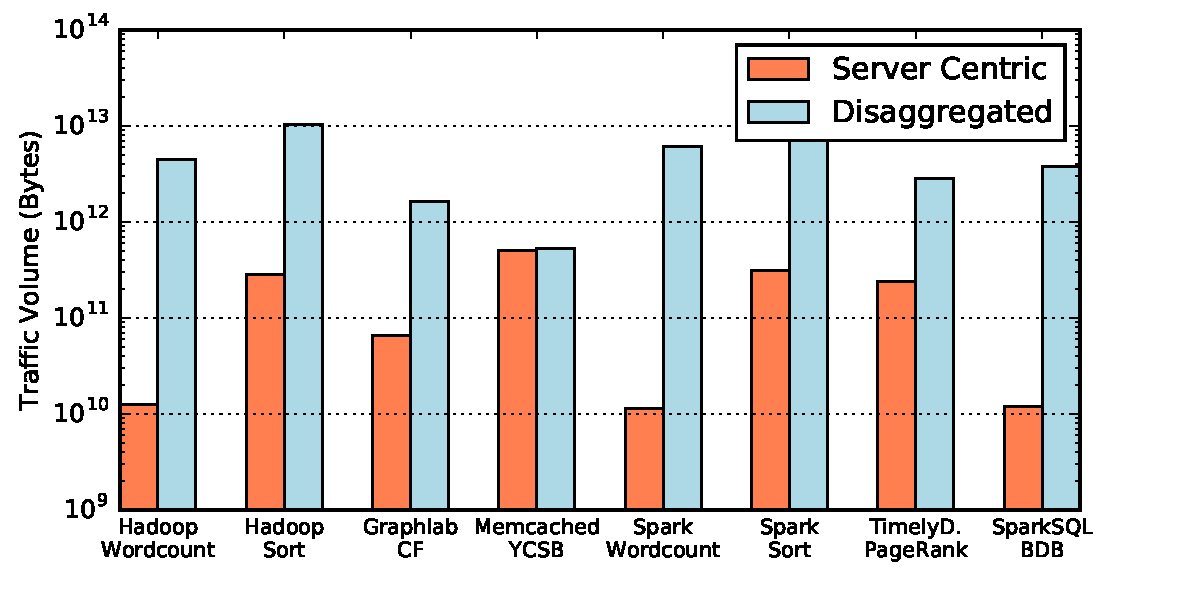
\includegraphics[width=0.95\columnwidth]{img/trafficVolume/trafficvolumes}
        \label{fig:trafvol:trafvols}
    }
    \subfigure[Temporal Traffic Volume Distribution]{
        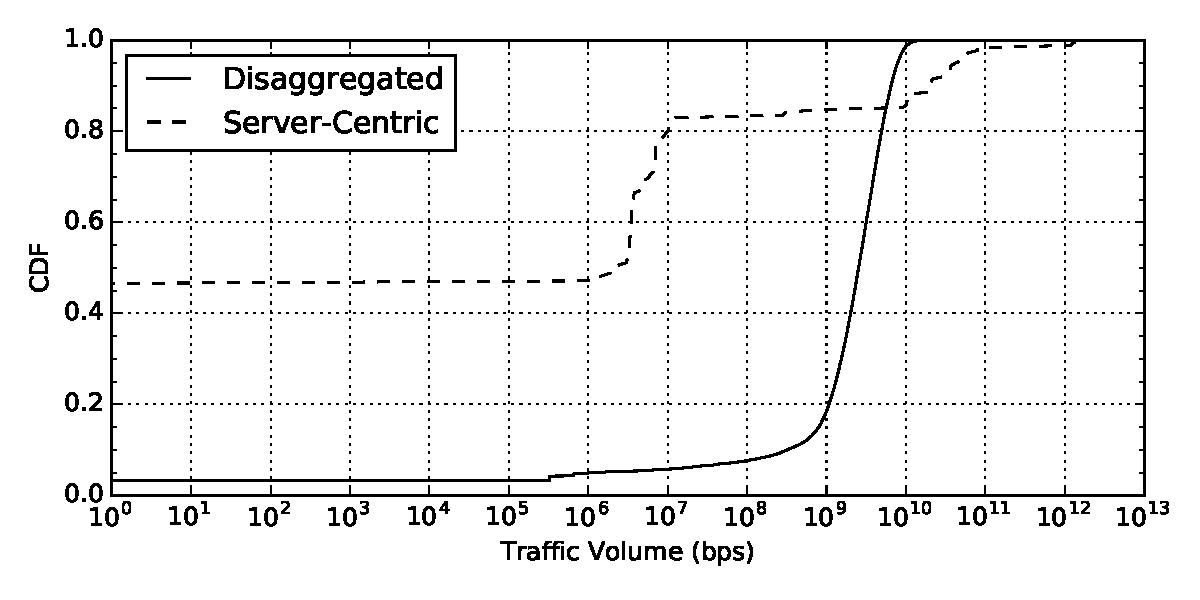
\includegraphics[width=0.95\columnwidth]{img/trafficVolume/temporalTraffic_cdf}
        \label{fig:trafvol:trafcdf}
    }
    \caption{\small{
    Figure~\ref{fig:trafvol:trafvols} compares traffic volumes between server centric and disaggregated datacenters. In almost all cases, the traffic volume increases by 1-2 orders of magnitude when moving from a server-centric to a disaggregated model; intuitively, CPU-memory and CPU-disk traffic that was previously contained within a server is now carried over the network. The obvious exception is memcached -- since most of the traffic in server-centric memcached corresponds to DRAM accesses, the traffic volume does not significantly increase.
    Figure~\ref{fig:trafvol:trafcdf} shows the distribution of traffic volumes for 100ms time intervals on the most highly loaded host while running the Spark Sort application. Note that for the disaggregated workload, the load over time is higher with disaggregation, but the tail load is lesser. Indeed, in the server centric workload, for almost half of the time intervals the link is quiescent.
    }}
    \label{fig:trafvol}
\end{figure*}
%

\subsection{Methodology: \dis Traffic Workloads}
\label{ssec:ssmethod-traffic}

%\paragraphb{Traces}
Using our experimental setup from \S\ref{ssec:rmethod},%, including the applications, datasets, and EC2 cluster (with VPC enabled). 
we collect three types of traces: 
%\vspace{-0.5em}
\begin{itemize}
\item \emph{`remote' memory accesses:} using our instrumentation that intercepts 
page faults as described in \S\ref{ssec:rmethod}; we record the 
request size in number of pages and the timestamp for each request.
%into the server's portion of the main memory that we've identified as ``remote memory''
\item \emph{network accesses:} we capture inter-machine traffic using {\tt tcpdump}~\cite{tcpdump}. {\tt tcpdump} gives us a packet-level log containing the five tuple for each packet. We treat all packets with the same five-tuple (protocol ID, source and destination address/port) as a single flow{\footnote{Applications choose one of the source ports randomly to establish a connection to the destination for each request. Given the large number of available ports, we assume that multiple connections between a pair of servers do not share the same port.  
One exception is memcached which uses long-lived connections (all packets between a client-server pair have the same five-tuple). In this case, we simply assumed each key-value pair lookup to be one flow.}}.
\item \emph{disk accesses:} we record application-level disk accesses using the {\tt blktrace} utility, which records a collection of (block\_start\_address, \#blocks, timestamp) tuples for each disk access request. 
%we don't do this 50us combination anymore
%Note that a single application-level file request may generate multiple such tuples since the data is not necessarily stored on consecutive disk blocks. Since {\tt blktrace} records accesses at the granularity of disk blocks, we must identify which tuples correspond to the same application-level request. This could be done by instrumenting the application; however, this is not only complex but also would potentially interfere with the application's performance. Instead, we simply assume that all tuples with timestamps within $50\mu$s correspond to the same application-level request. 
%The only difference is that we enabled the Virtual Private Network (VPC) in our cluster, ensuring no interference with other Amazon EC2 machines. 
\end{itemize} 

Next, we translate the accesses from the above traces to network flows 
in our simulated disaggregated cluster. 
%\paragraphb{Mapping accesses to network flows in \dis}
%Mapping the above traces to network traffic in our emulated disaggregated cluster again 
This involves two steps. 
First, we must define the resource blades that form our endpoints in the disaggregated cluster (i.e., map the resources in our server-based cluster into standalone blades in a disaggregated cluster) and then map the above traces to flows between these endpoints. 
Mapping resources to blades is straightforward; each server is split into one compute blade, one memory blade, and one storage blade.
%We don't do the below 3 disk thing either anymore
%We assume one server maps to one compute blade and one memory blade but consolidate disk resources from different servers into a smaller number of disk blades so as to compensate for the relatively low throughput to disk (doing otherwise would only decrease our network load); specifically, we assume that one server's disk resources map to $60\%$ of a standalone disk blade.\footnote{We arrived at this number by aiming to balance network and disk throughputs while maintaining sufficient redundancy.} 

Having defined our resource blades as above, we now define how traffic 
flows between them. 
All memory and disk accesses captured above are associated with a specific address in the corresponding CPU's global virtual address space. We assume this address space is uniformly partitioned across all memory and disk blades reflecting our assumption of distributed data placement (\S\ref{ssec:system}).  
%This address space is partitioned across five memory blades and three disk blades{\footnote{Some of the disk space was not utilized in our cluster.}} in \dis using range partitioning. 
%distributes data across memory or disk access in our EC2 cluster may now be mapped along multiple blades.

One subtlety remains. Consider the disk accesses at a server A in the original cluster: one might view all these disk accesses as corresponding to a flow between the compute blade corresponding A and the disk blade corresponding to A but in reality some of these disk accesses may have been issued by A's CPU in response to a request from a remote server B (\eg, due to a shuffle request). 
In the disaggregated cluster, this access should be treated as a network flow between \emph{B}'s compute blade and A's disk blade (i.e., the 
compute blade obtained by disaggregating server B and the disk blade that corresponds to disaggregating A).


%The memory and disk requests using SIT and {\tt blktrace} are captured locally at each individual server. Some of these requests correspond to requests originating at remote CPUs (\eg, shuffle traffic). 

To correctly attribute accesses to the CPU that originates the request, we 
match network and disk traces across the cluster -- e.g., matching the network traffic between B and A to the disk traffic at A -- using a heuristic based on both the timestamps and volume of data transferred. 
%perform a timestamp-based matching between requests captured at each individual server, and inter-machine NIC traffic from {\tt tcpdump}. 
If a locally captured memory or disk access request matches a local flow in our {\tt tcpdump} traces, then it is assumed to be part of a remote read and is attributed to the remote endpoint of the network flow.
%(more than $85\%$, on an average, were correctly attributed in our evaluation). 
Otherwise, the memory/disk access is assumed to have originated from the local CPU. 
%generated locally. 


Figure~\ref{fig:trafvol} plots a few characteristics of our resultant \dis traffic workload alongside that in the corresponding non-disaggregated architecture. As expected, disaggregation significantly changes the nature of the traffic workload, pointing to the importance of our characterization effort.




\subsection{Methodology: Queueing delay}
\label{ssec:ssmethod}

We evaluate the use of existing network designs for \dis in two steps.
First, we evaluate how existing network designs fare under \dis traffic workloads. 
For this, we consider a suite of state-of-the-art network designs and use simulation to evaluate their network-layer performance -- measured in terms of flow completion time (FCT) -- under the traffic workloads we generate as above.
%corresponding to each of our applications.
%from (\S\ref{sec:workloads}).
We then return to actual execution of our applications (Table~\ref{tab:workloads}) and once again emulate disaggregation by injecting latencies for page misses. 
However, now we inject the flow completion times obtained from our best-performing network design (as opposed to the constant latencies from \S\ref{sec:requirements}). This last step effectively `closes the loop', allowing us to evaluate the impact of disaggregation on application-level performance for realistic network designs and conditions. 


%
% \begin{figure*}
% \centering
% \sbox{\measurebox}{%
%   \begin{minipage}[b]{0.45\textwidth}
%   \subfloat
%     {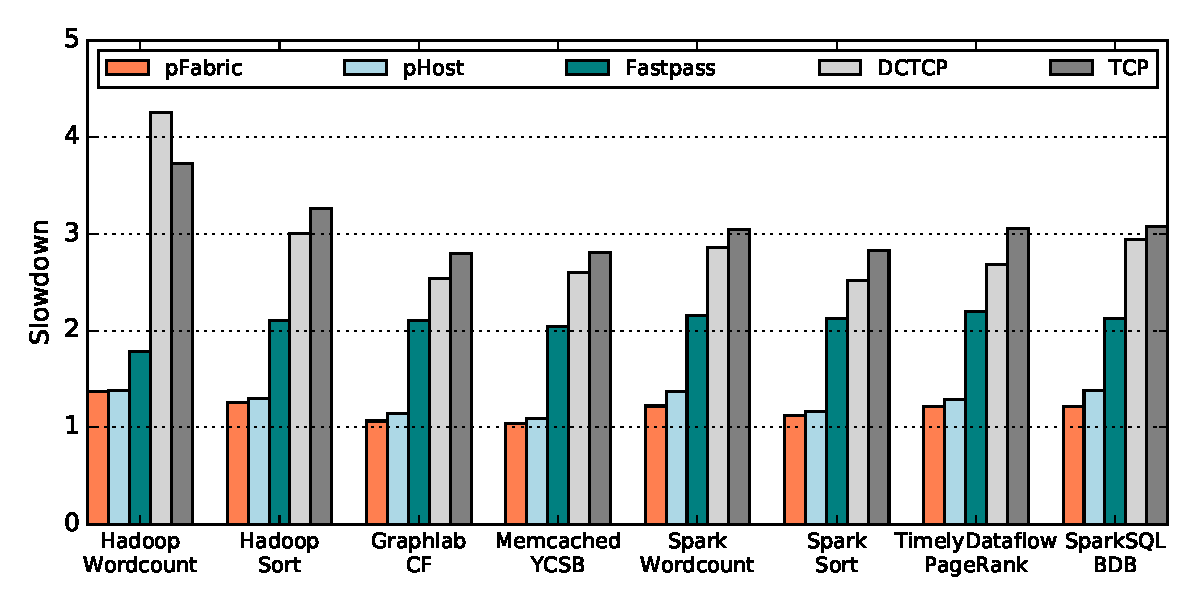
\includegraphics[width=\textwidth,height=5cm]{img/slowdowns/100g/allFlows_dc-scale_slowdowns}}
%   \end{minipage}}
% \usebox{\measurebox}\qquad
% \begin{minipage}[b][\ht\measurebox][s]{.45\textwidth}
% \centering
% \subfloat
%   {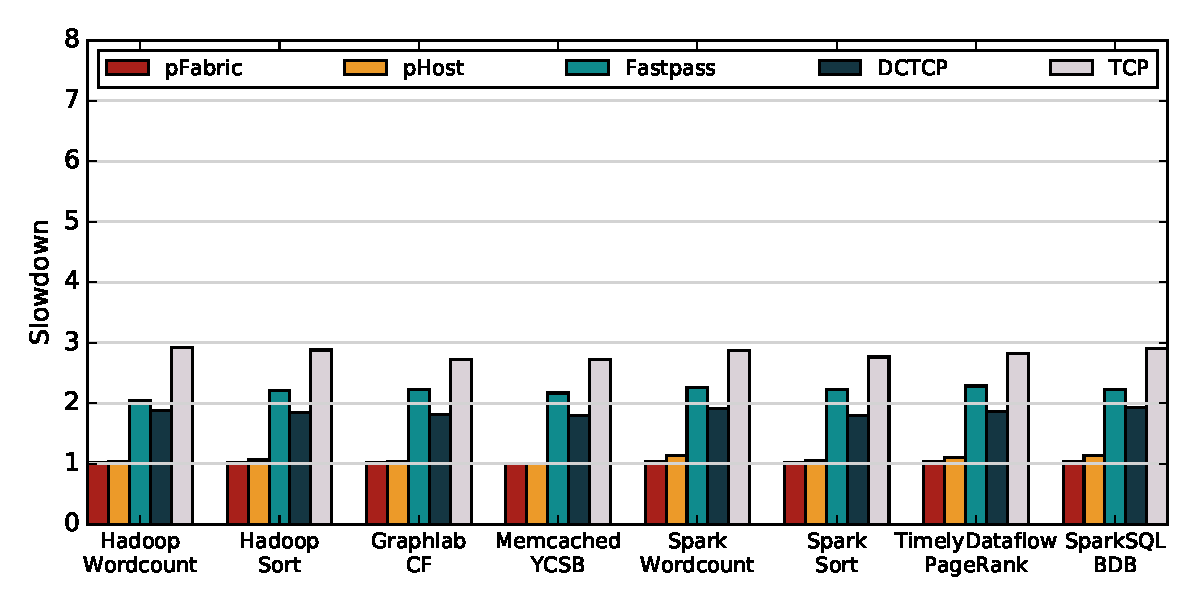
\includegraphics[width=\textwidth,height=2cm]{img/slowdowns/100g/smallFlows_dc-scale_slowdowns}}

% \vfill

% \subfloat
%   {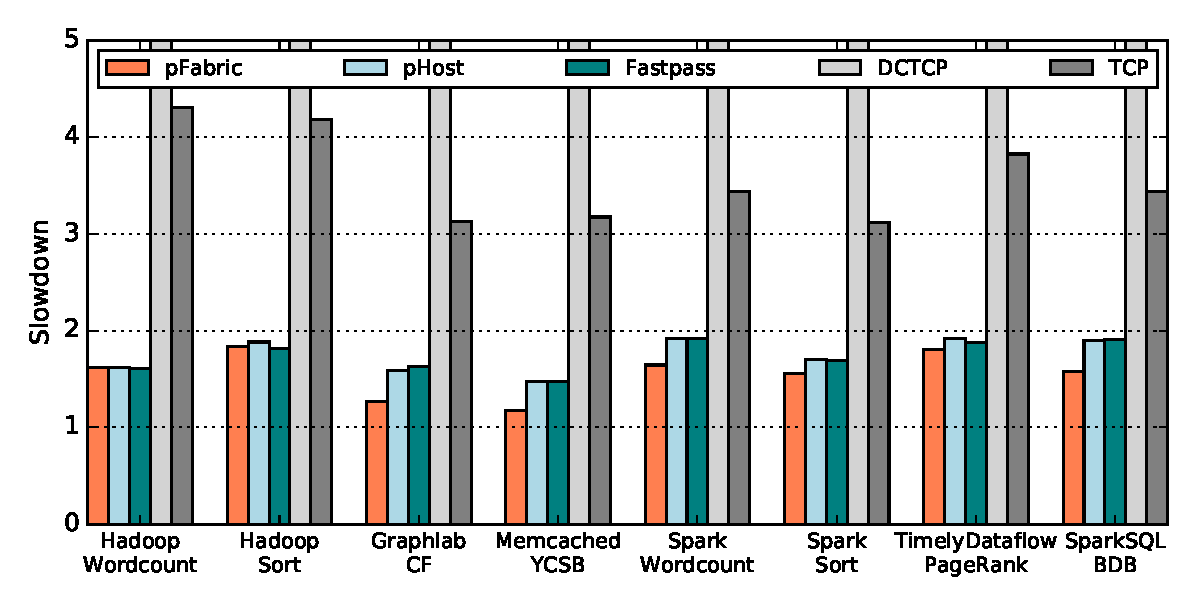
\includegraphics[width=\textwidth,height=2cm]{img/slowdowns/100g/bigFlows_dc-scale_slowdowns}}
% \end{minipage}
% \caption{\small{The mean slowdown for pFabric, pHost, Fastpass, DCTCP, and TCP for each of the eight applications at datacenter-scale: (top) overall; (left) short flows only; (right) long flows.}}
% \label{fig:phostp-ds}
% \end{figure*}



%\begin{figure*}
%   \centering
%     \subfigure{
%       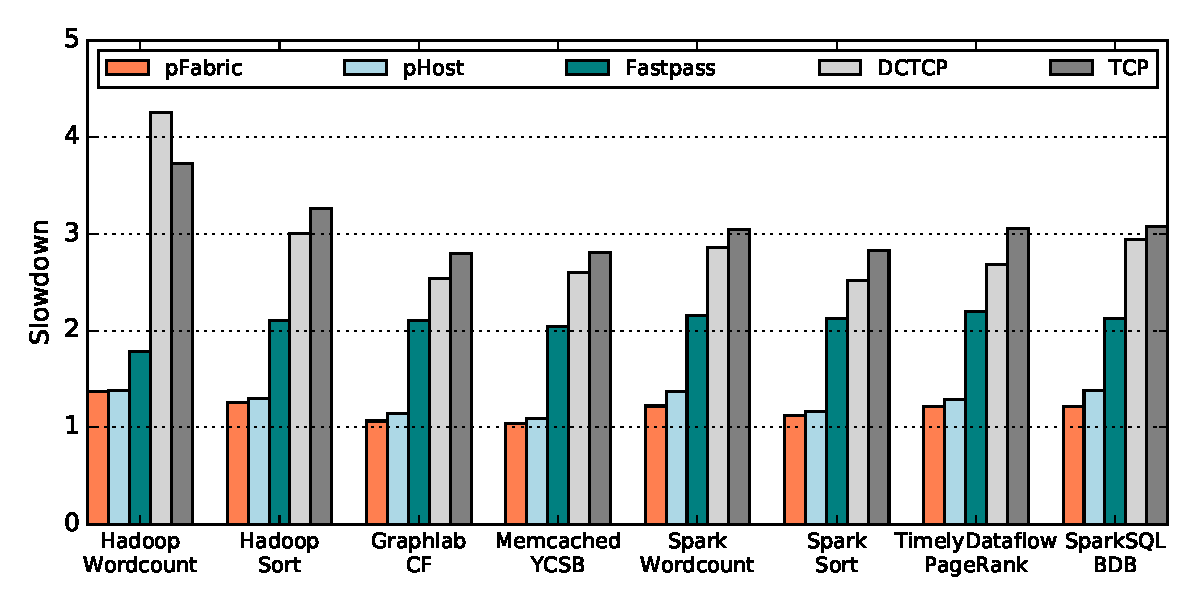
\includegraphics[width = 4in]{img/slowdowns/100g/allFlows_dc-scale_slowdowns} 
%     }
    
%     \subfigure{
%     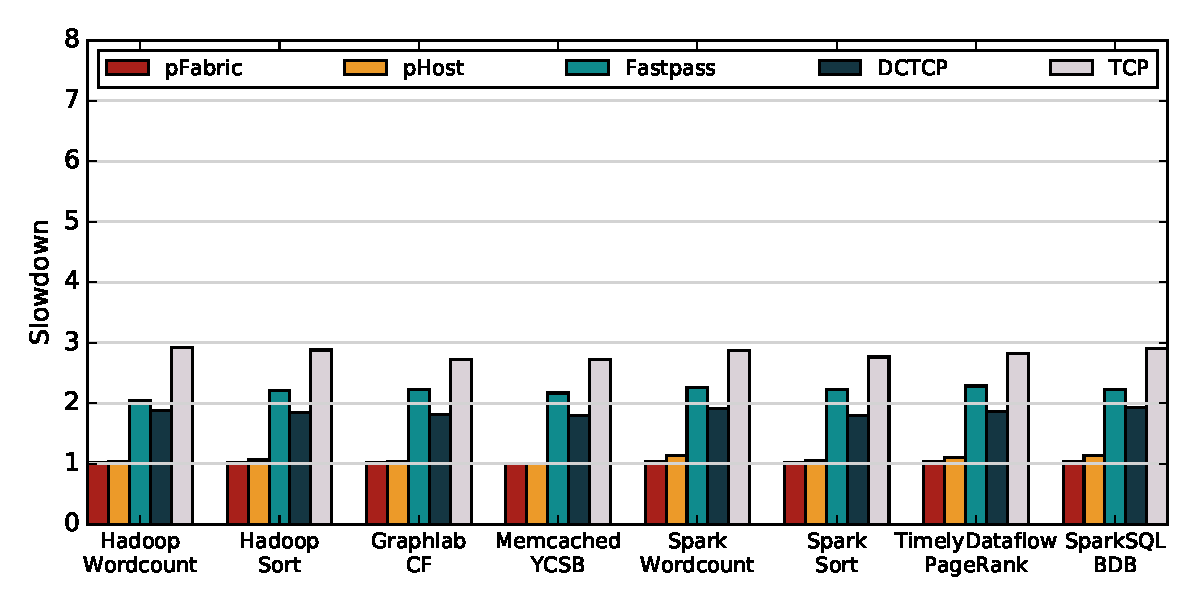
\includegraphics[width=2in]{img/slowdowns/100g/smallFlows_dc-scale_slowdowns}
%     }
%     \subfigure{
%     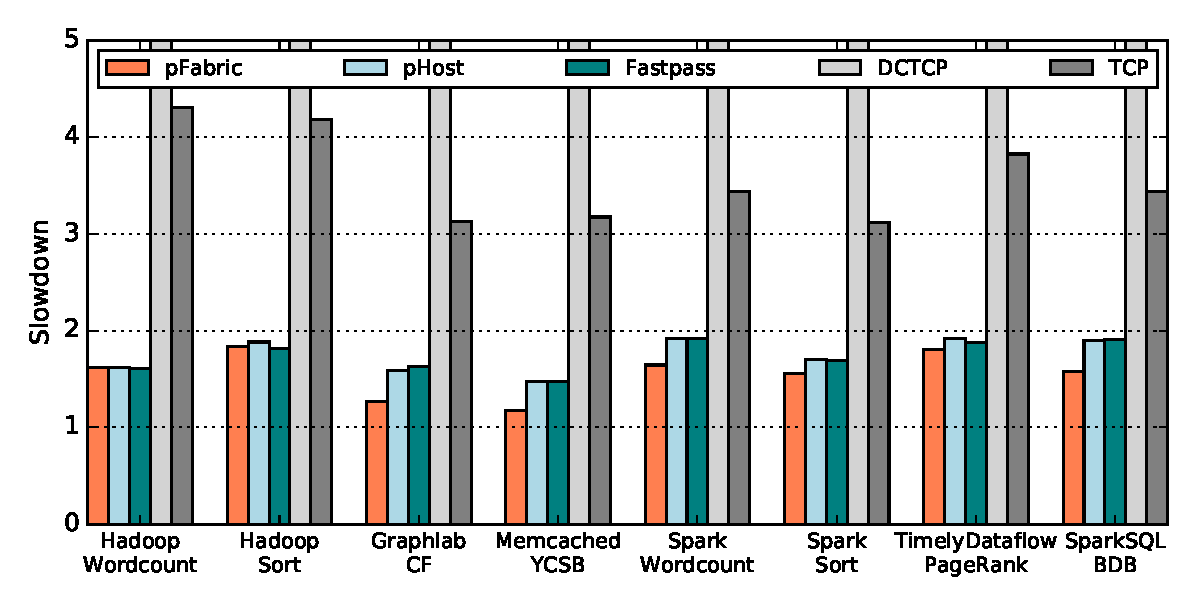
\includegraphics[width=2in]{img/slowdowns/100g/bigFlows_dc-scale_slowdowns}
%     }
%   \caption{\small{The mean slowdown for pFabric, pHost, Fastpass, DCTCP, and TCP for each of the eight applications at datacenter-scale: (top) overall; (left) short flows only; (right) long flows.}}
%   \label{fig:phostp-ds}
% \end{figure*}
%



% \begin{figure*}
% \centering
% \sbox{\measurebox}{%
%   \begin{minipage}[b]{0.45\textwidth}
%   \subfloat
%     {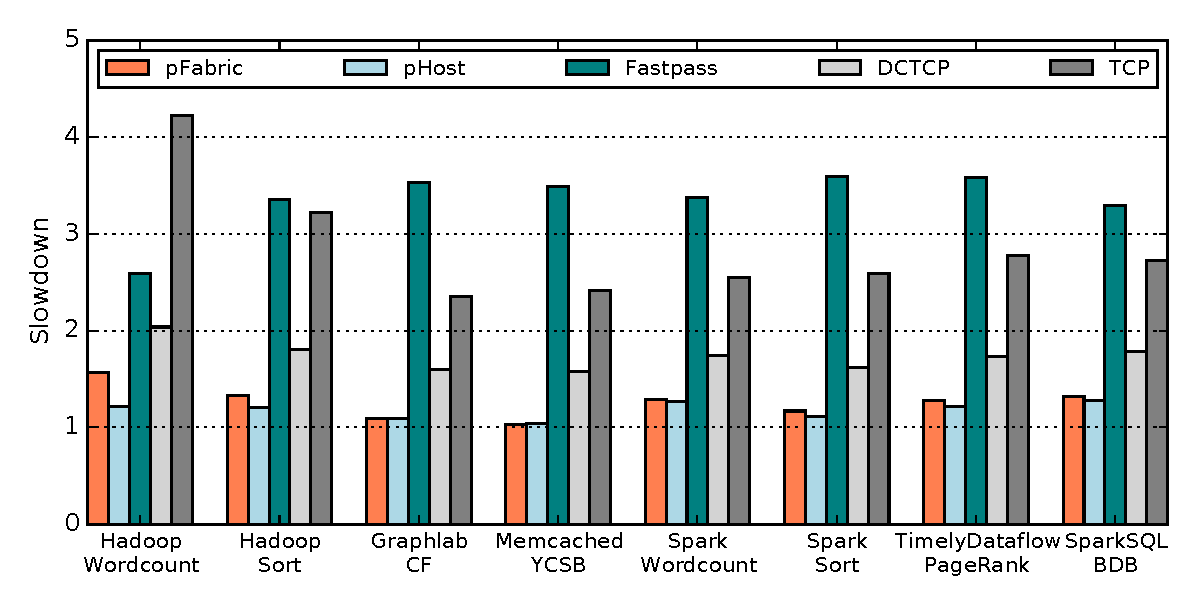
\includegraphics[width=\textwidth,height=5cm]{img/slowdowns/100g/allFlows_rack-scale_slowdowns}}
%   \end{minipage}}
% \usebox{\measurebox}\qquad
% \begin{minipage}[b][\ht\measurebox][s]{.45\textwidth}
% \centering
% \subfloat
%   {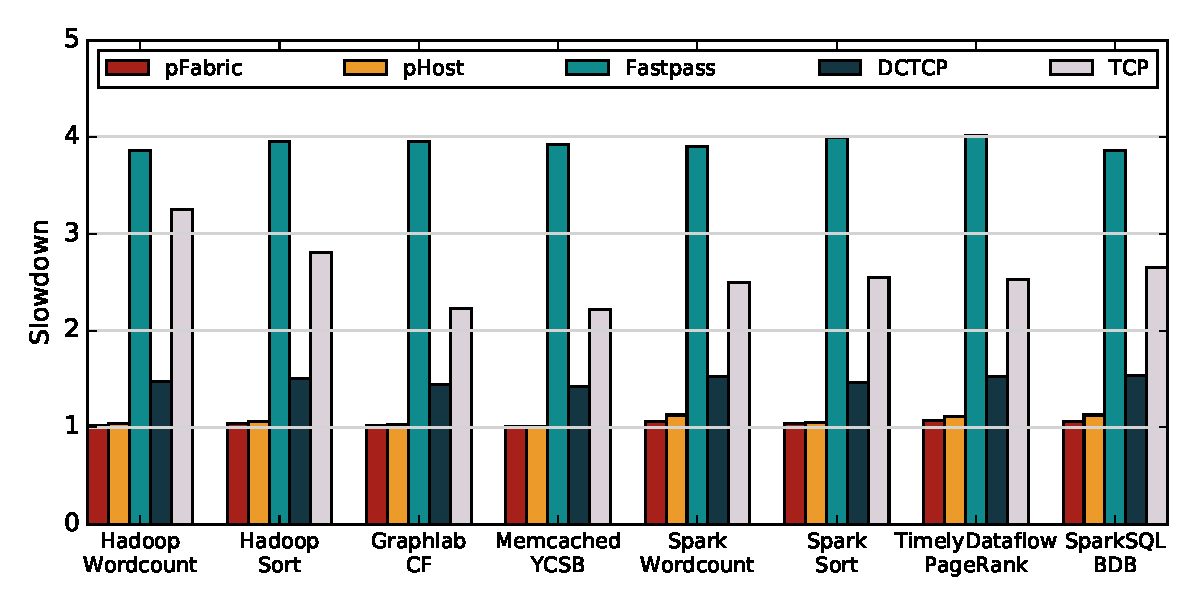
\includegraphics[width=\textwidth,height=2cm]{img/slowdowns/100g/smallFlows_rack-scale_slowdowns}}

% \vfill

% \subfloat
%   {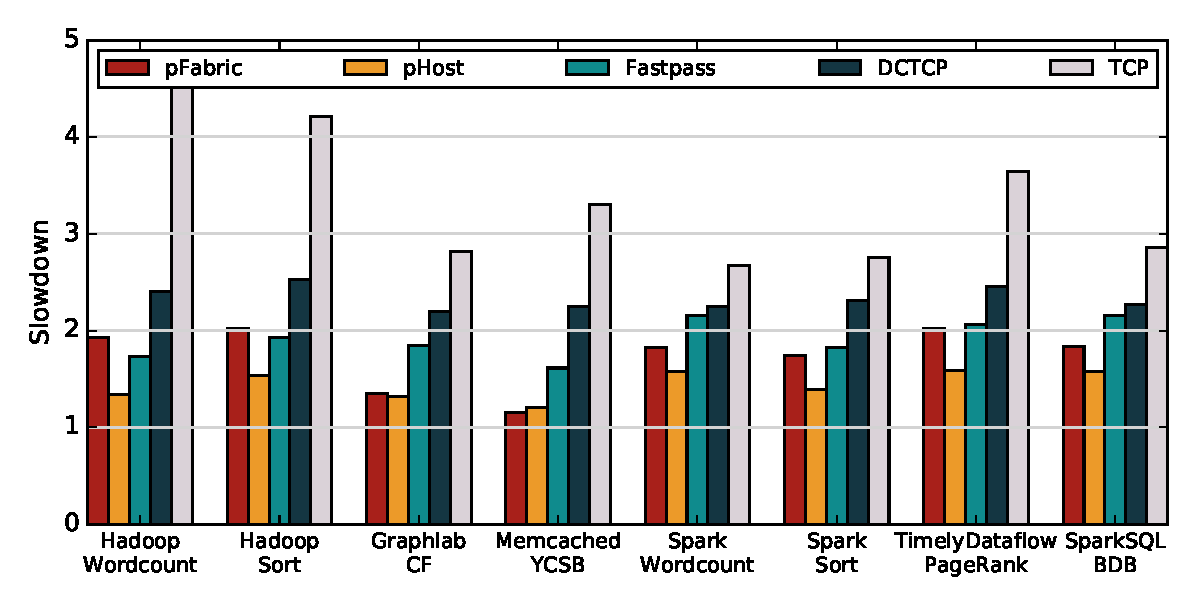
\includegraphics[width=\textwidth,height=2cm]{img/slowdowns/100g/bigFlows_rack-scale_slowdowns}}
% \end{minipage}
% \caption{\small{The mean slowdown for pFabric, pHost, Fastpass, DCTCP, and TCP for each of the eight applications at rack-scale: (top) overall; (left) short flows only; (right) long flows.}}
% \label{fig:phostp-rs}
% \end{figure*}


% \begin{figure*}
%   \centering
%     \subfigure{
%       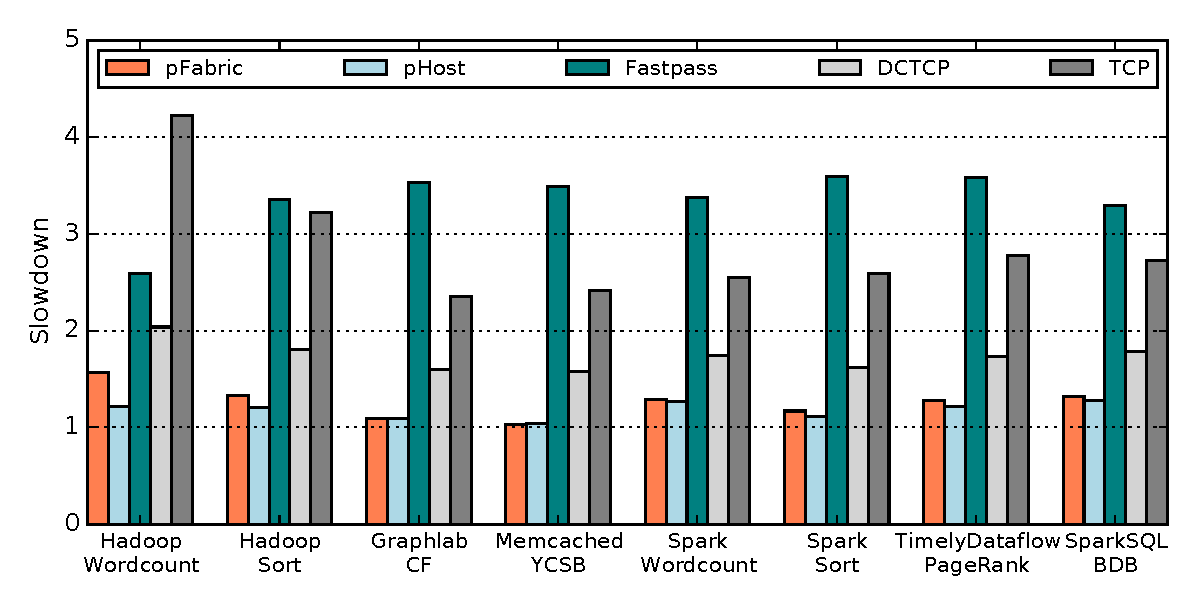
\includegraphics[width = 4in]{img/slowdowns/100g/allFlows_rack-scale_slowdowns} 
%     }
    
%     \subfigure{
%     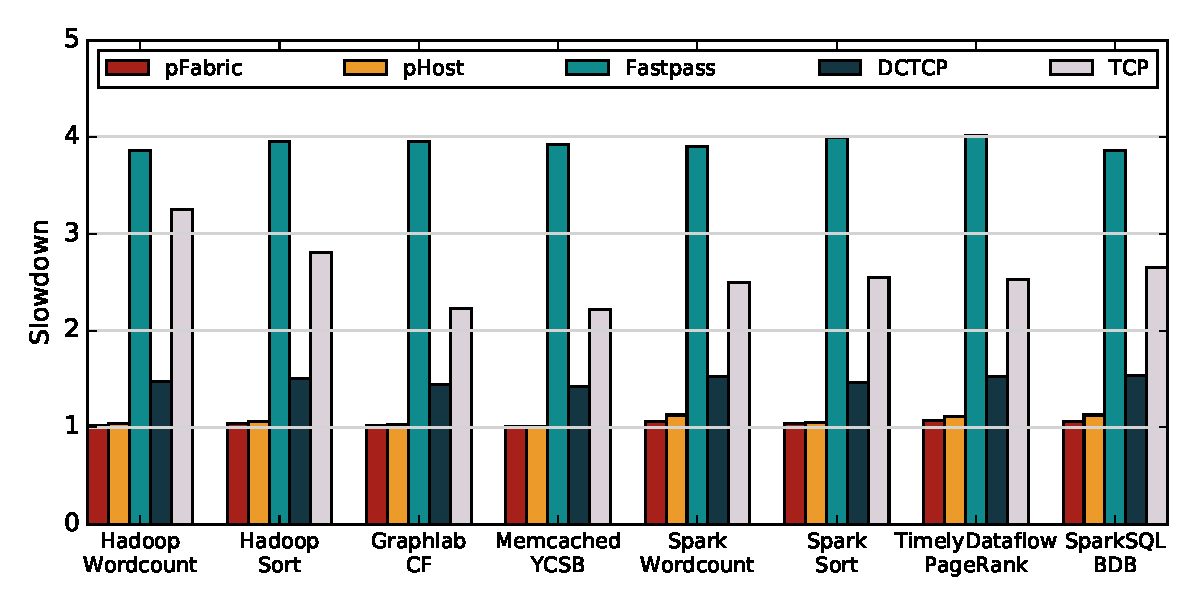
\includegraphics[width=2in]{img/slowdowns/100g/smallFlows_rack-scale_slowdowns}
%     }
%     \subfigure{
%     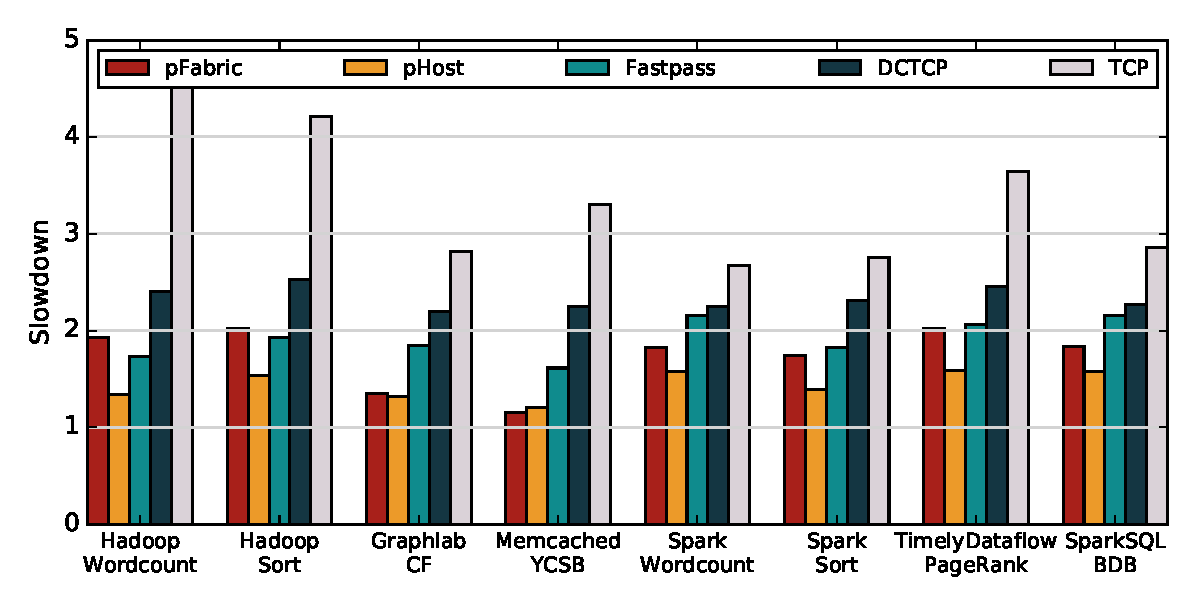
\includegraphics[width=2in]{img/slowdowns/100g/bigFlows_rack-scale_slowdowns}
%     }
%   \caption{\small{The mean slowdown for pFabric, pHost, Fastpass, DCTCP, and TCP for each of the eight applications at rack-scale: (top) overall; (left) short flows only; (right) long flows.}}
%   \label{fig:phostp-rs}
% \end{figure*}


% \begin{figure*}
% \centering
% \sbox{\measurebox}{%
%   \begin{minipage}[b]{0.45\textwidth}
%   \subfloat
%     {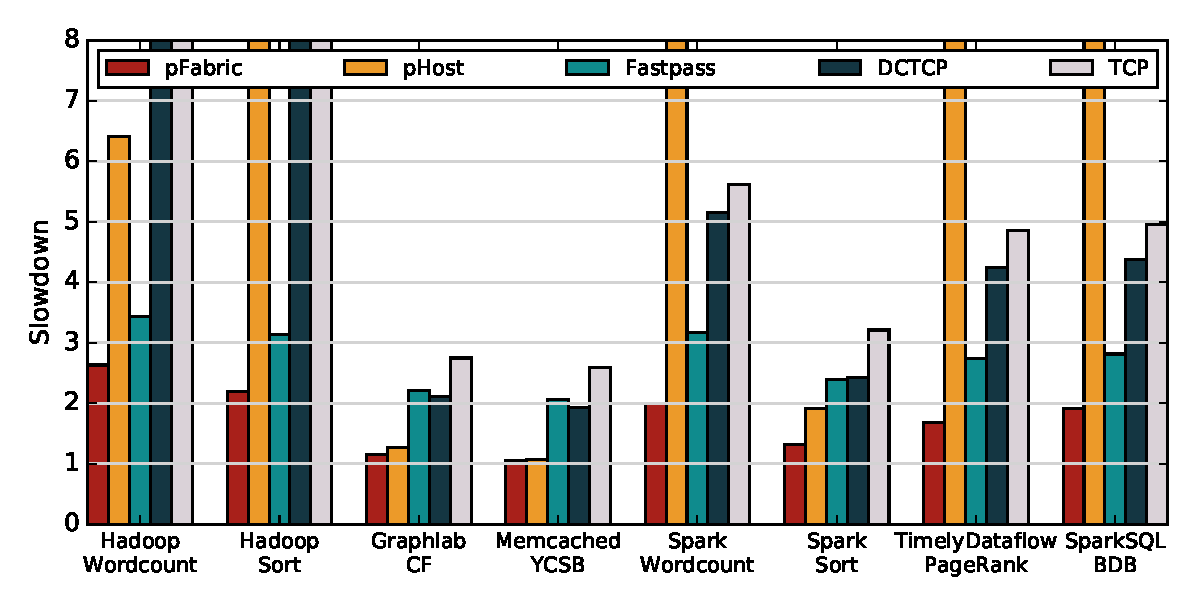
\includegraphics[width=\textwidth,height=5cm]{img/slowdowns/40g/allFlows_dc-scale_slowdowns}}
%   \end{minipage}}
% \usebox{\measurebox}\qquad
% \begin{minipage}[b][\ht\measurebox][s]{.45\textwidth}
% \centering
% \subfloat
%   {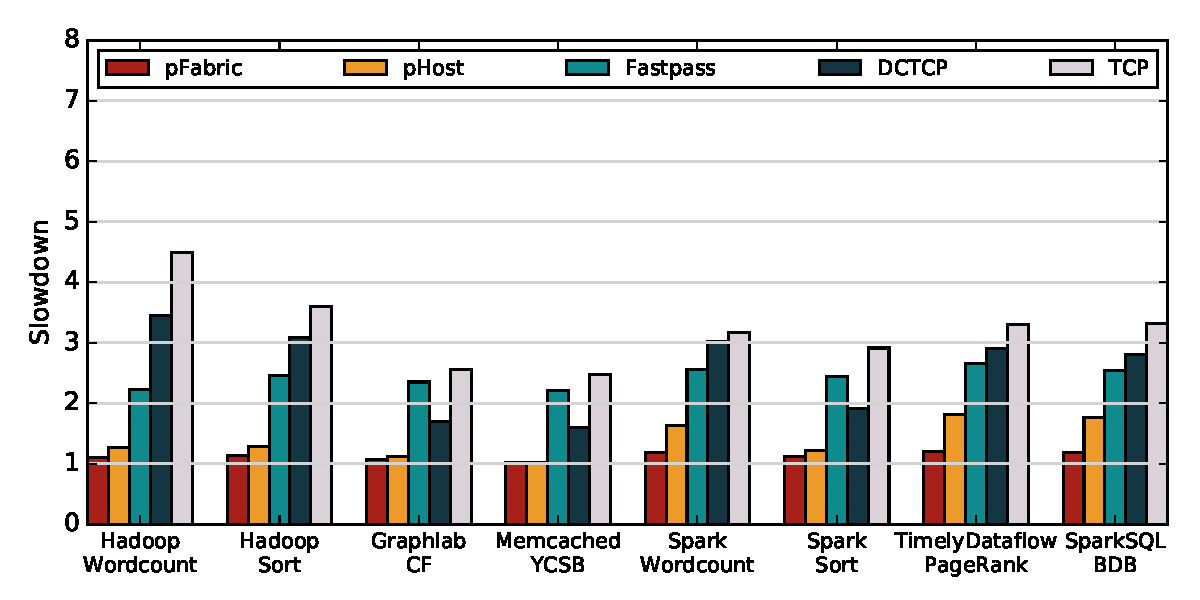
\includegraphics[width=\textwidth,height=2cm]{img/slowdowns/40g/smallFlows_dc-scale_slowdowns}}

% \vfill

% \subfloat
%   {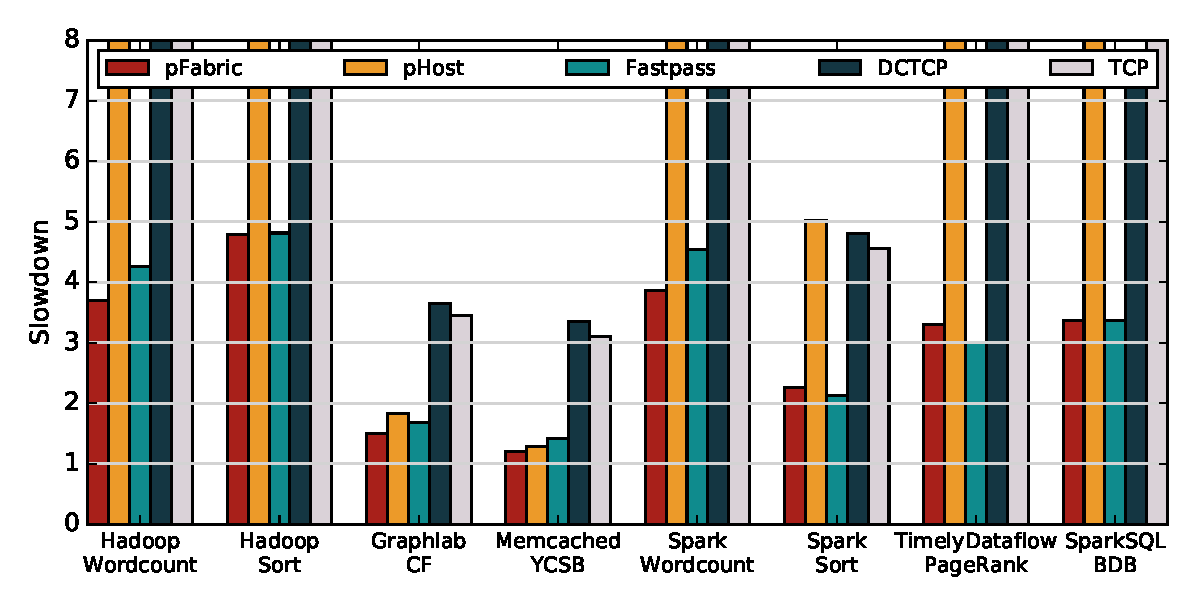
\includegraphics[width=\textwidth,height=2cm]{img/slowdowns/40g/bigFlows_dc-scale_slowdowns}}
% \end{minipage}
% \caption{\small{The mean slowdown at 40g for pFabric, pHost, Fastpass, DCTCP, and TCP for each of the eight applications at datacenter-scale: (top) overall; (left) short flows only; (right) long flows.}}
% \label{fig:phostp-ds-40g}
% \end{figure*}


% \begin{figure*}
%   \centering
%     \subfigure{
%       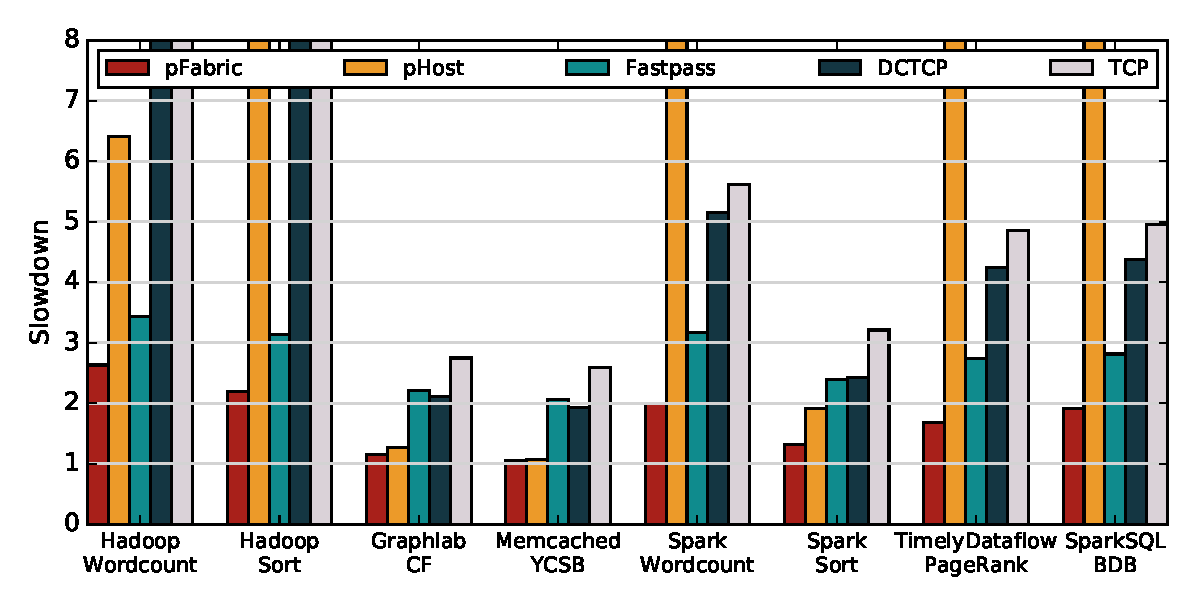
\includegraphics[width = 4in]{img/slowdowns/40g/allFlows_dc-scale_slowdowns} 
%     }
    
%     \subfigure{
%     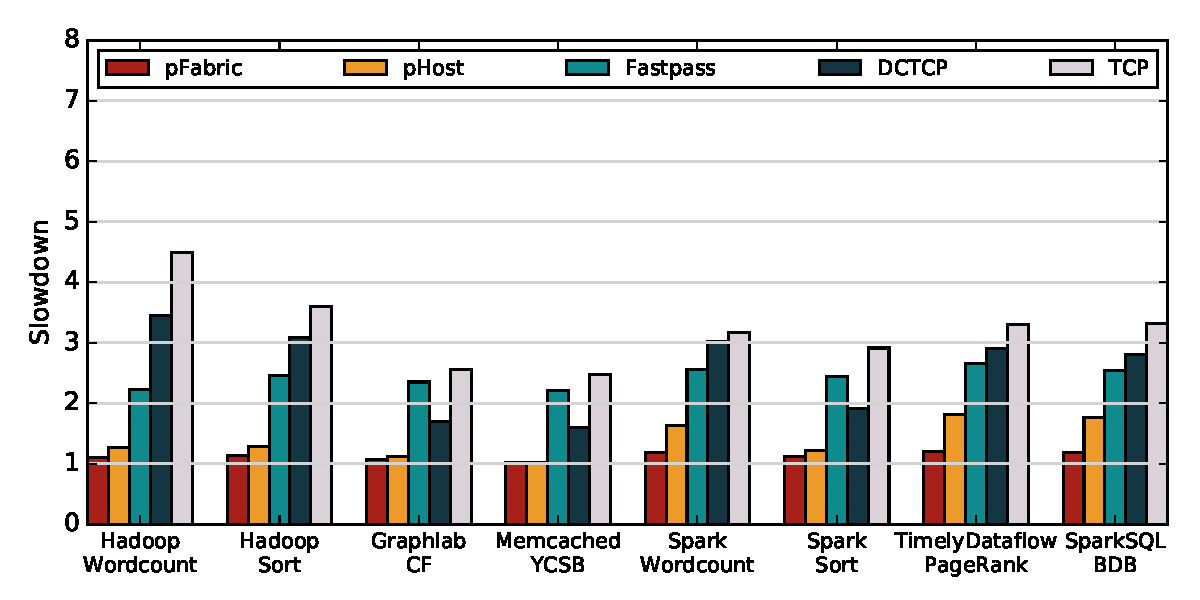
\includegraphics[width=2in]{img/slowdowns/40g/smallFlows_dc-scale_slowdowns}
%     }
%     \subfigure{
%     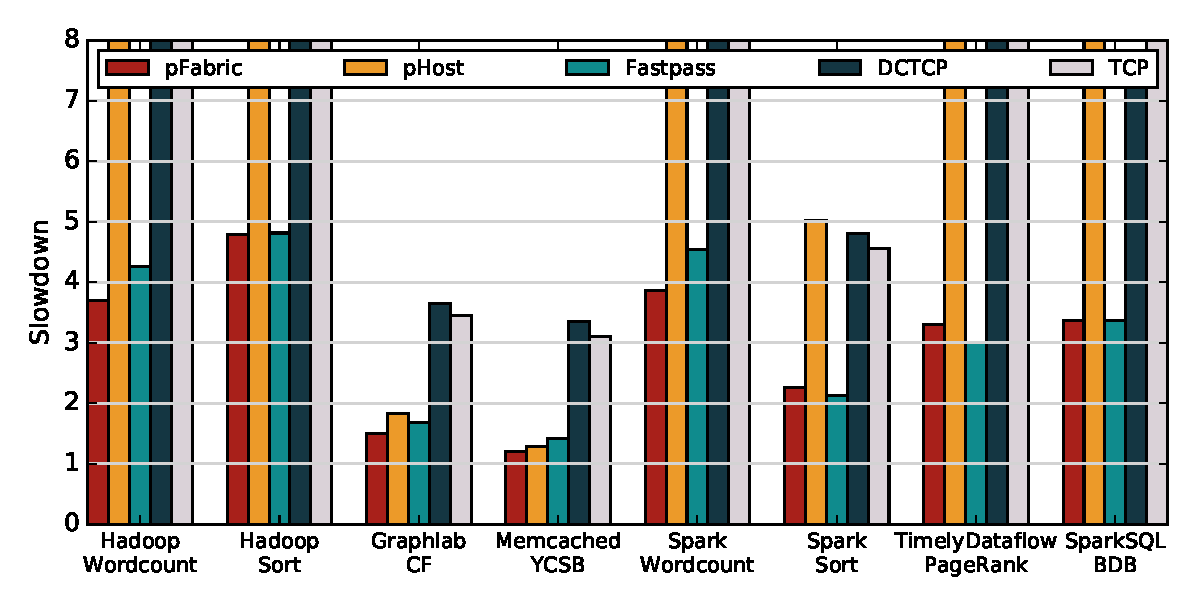
\includegraphics[width=2in]{img/slowdowns/40g/bigFlows_dc-scale_slowdowns}
%     }
%   \caption{\small{The mean slowdown at 40g for pFabric, pHost, Fastpass, DCTCP, and TCP for each of the eight applications at datacenter-scale: (top) overall; (left) short flows only; (right) long flows.}}
%   \label{fig:phostp-ds-40g}
% \end{figure*}
%

% \begin{figure*}
% \centering
% \sbox{\measurebox}{%
%   \begin{minipage}[b]{0.45\textwidth}
%   \subfloat
%     {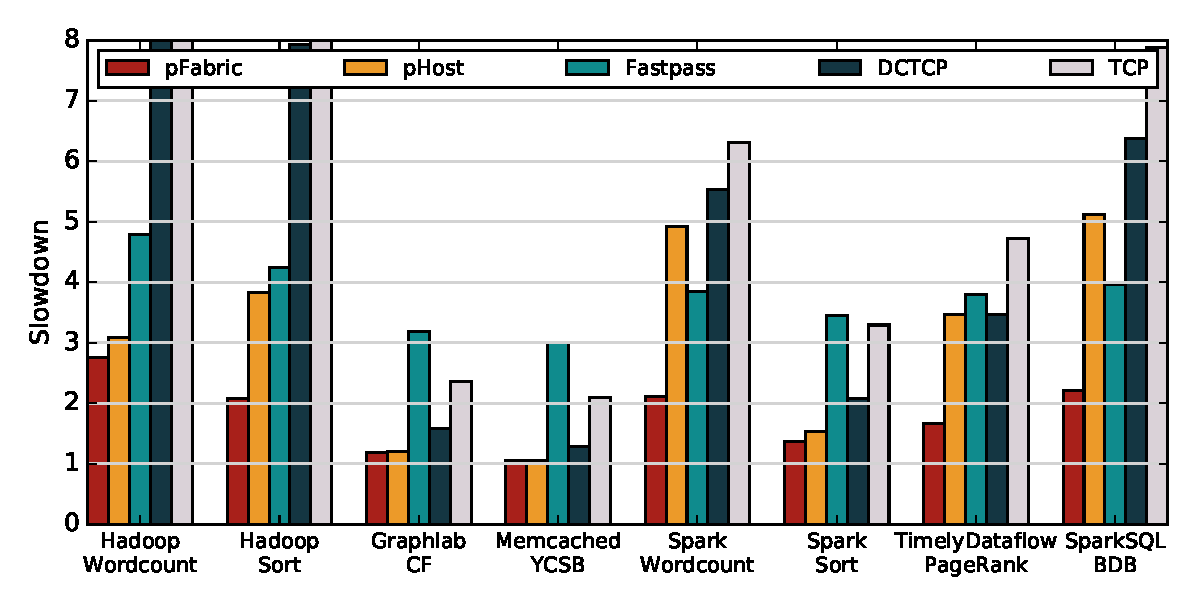
\includegraphics[width=\textwidth,height=5cm]{img/slowdowns/40g/allFlows_rack-scale_slowdowns}}
%   \end{minipage}}
% \usebox{\measurebox}\qquad
% \begin{minipage}[b][\ht\measurebox][s]{.45\textwidth}
% \centering
% \subfloat
%   {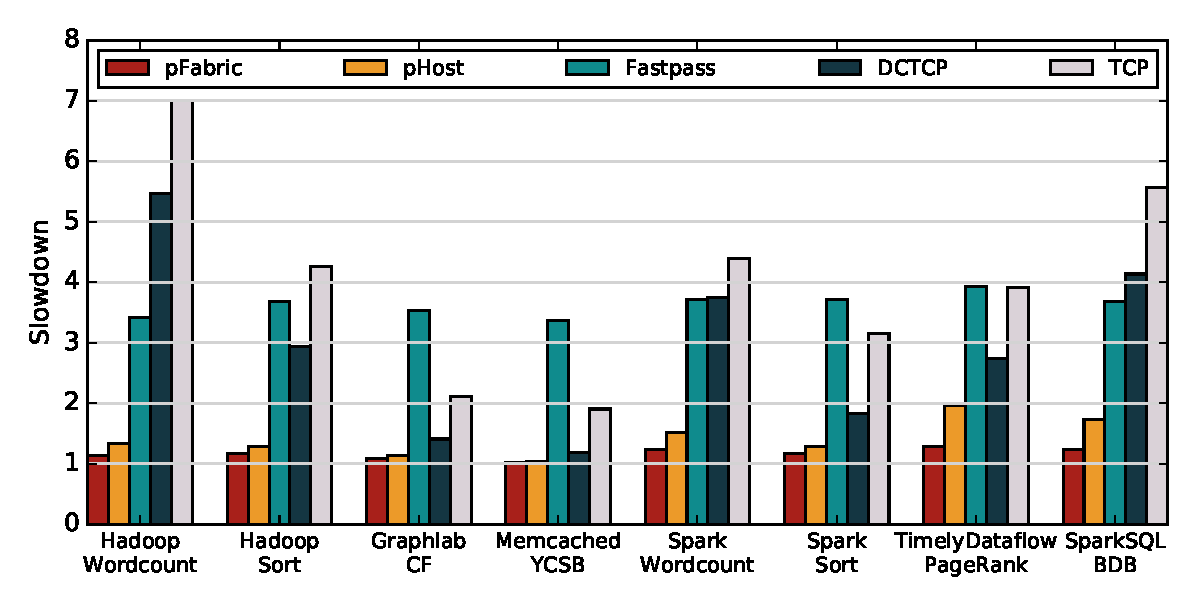
\includegraphics[width=\textwidth,height=2cm]{img/slowdowns/40g/smallFlows_rack-scale_slowdowns}}

% \vfill

% \subfloat
%   {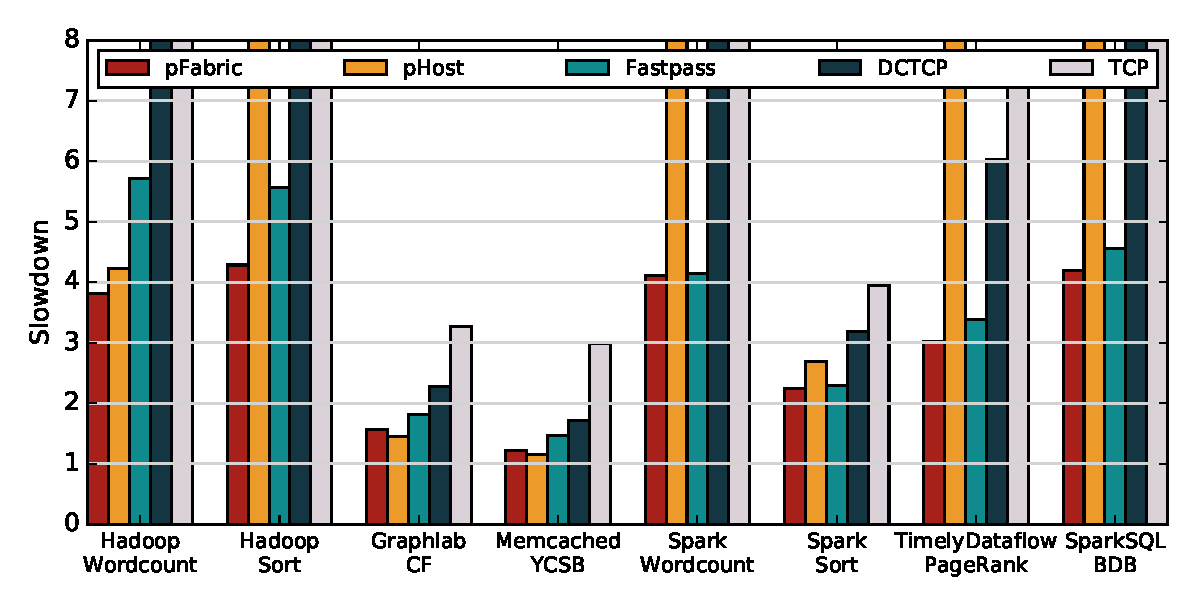
\includegraphics[width=\textwidth,height=2cm]{img/slowdowns/40g/bigFlows_rack-scale_slowdowns}}
% \end{minipage}
% \caption{\small{The mean slowdown at 40g for pFabric, pHost, Fastpass, DCTCP, and TCP for each of the eight applications at rack-scale: (top) overall; (left) short flows only; (right) long flows.}}
%   \label{fig:phostp-rs-40g}
% \end{figure*}


% \begin{figure*}
%   \centering
%     \subfigure{
%       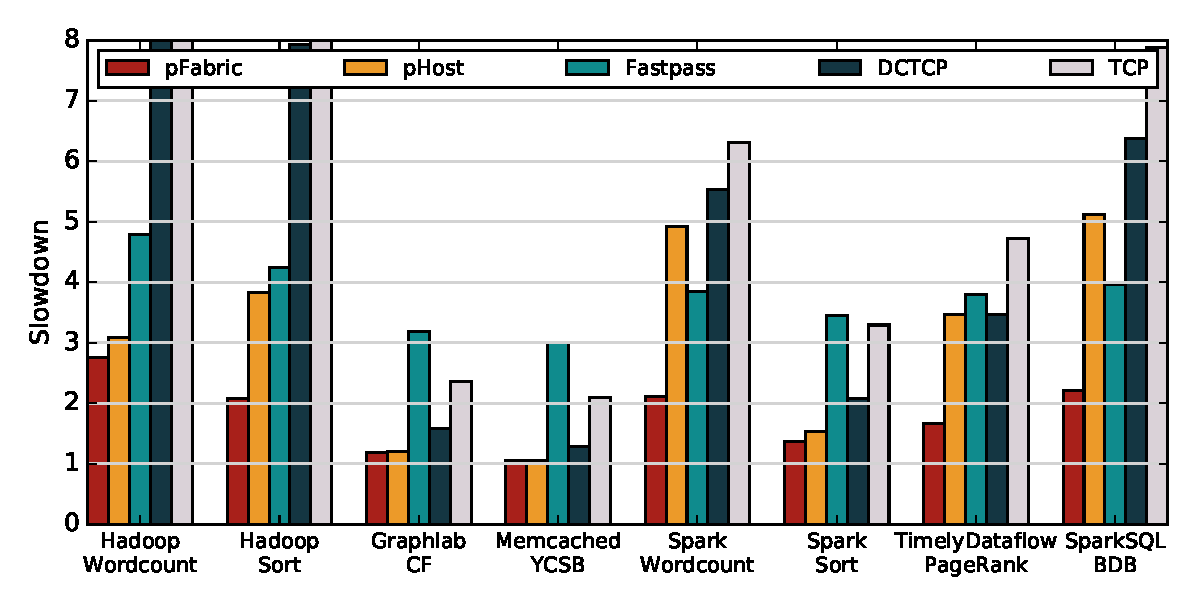
\includegraphics[width = 4in]{img/slowdowns/40g/allFlows_rack-scale_slowdowns} 
%     }
    
%     \subfigure{
%     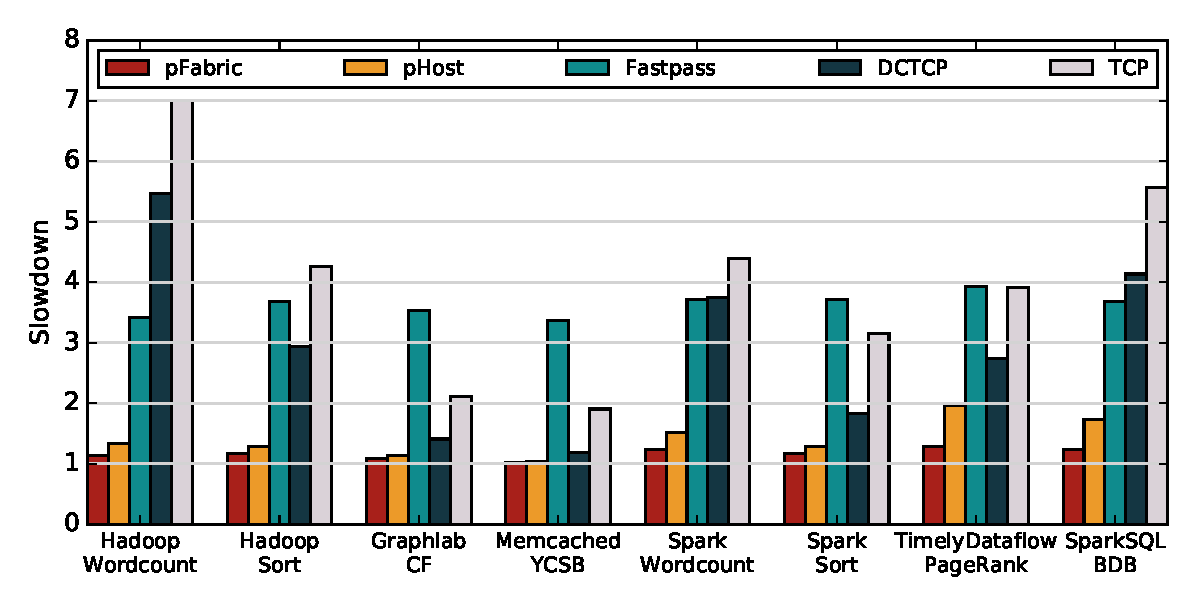
\includegraphics[width=2in]{img/slowdowns/40g/smallFlows_rack-scale_slowdowns}
%     }
%     \subfigure{
%     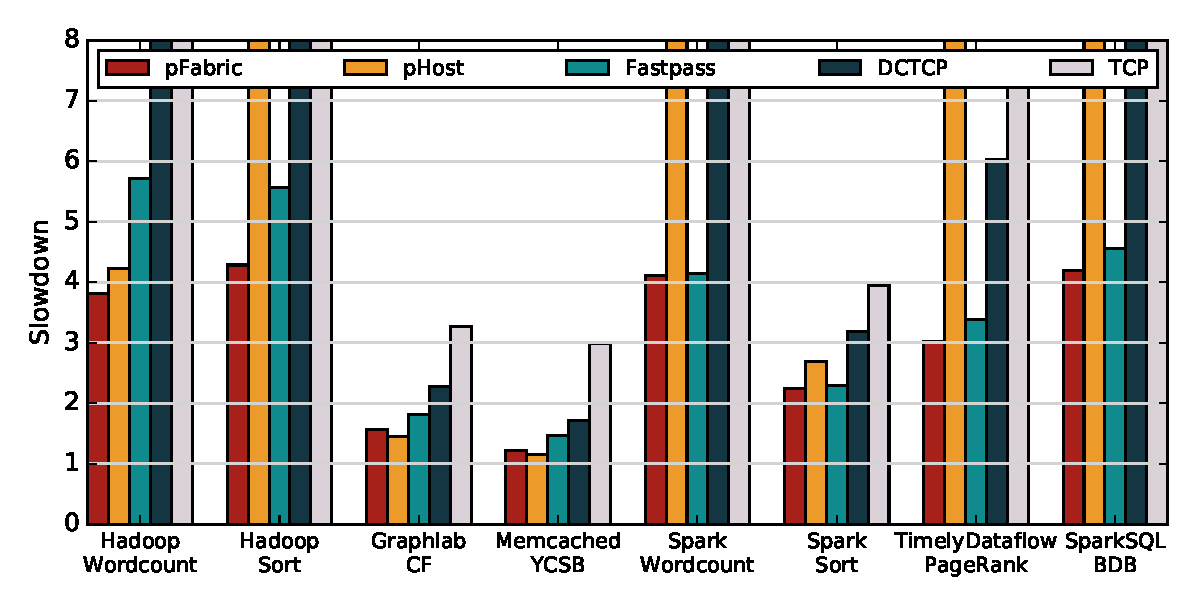
\includegraphics[width=2in]{img/slowdowns/40g/bigFlows_rack-scale_slowdowns}
%     }
%   \caption{\small{The mean slowdown at 40g for pFabric, pHost, Fastpass, DCTCP, and TCP for each of the eight applications at rack-scale: (top) overall; (left) short flows only; (right) long flows.}}
%   \label{fig:phostp-rs-40g}
% \end{figure*}

%There were multiple challenges in performing the above evaluations that we encountered.
%

\paragraphb{Simulation Setup}
For all the simulations in this section, we use the same setup as prior work on datacenter transport designs~\cite{pfabric, phost}. 
We simulate a %$144$-node (9 racks of 16 servers each) 
topology with 9 racks and a full bisection bandwidth Clos topology with $36$KB buffers per port; our two changes from prior work are to use $40$Gbps or $100$Gbps access links as per our discussion in~\S\ref{sec:requirements}, and setting propagation and switching delays as discussed in \S\ref{ssec:rtt} (Table~\ref{tab:latency}): 20 ns within a rack, 200ns for aggregation links, and a switching delay of 200ns per hop. 
We evaluate the following five protocols. 
%\an{not true? can we just say we took the default settings from the papers and adapted them to our BDP?: } 
In each case, we set protocol-specific parameters following the default settings but adapted to our bandwidth-delay product as recommended. 
%to the values that we found (through experimentation) yielded the best performance for that protocol.

\begin{enumerate}[leftmargin=*]
\itemsep0em
\item {\bf TCP}, with an initial congestion window of 2.
\item {\bf DCTCP}, which leverages ECN for enhanced performance in datacenter contexts.  
\item {\bf pFabric}, approximates shortest-job-first scheduling in a network context using switch support to prioritize  flows with a smaller remaining flow size~\cite{pfabric}. We set pFabric to have an initial congestion window of 12 packets and a retransmission timeout of $45$us.
%
\item {\bf pHost}, emulates pFabric's behavior but using only scheduling at the end hosts~\cite{phost} and hence allows the use of commodity switches. We set pHost to have a free token limit of 8 packets and a retransmission timeout of $9.5$us as recommended in ~\cite{phost}.
%; we obtained these parameters from pHost's implementation.
%
\item {\bf Fastpass}, introduces a centralized scheduler that schedules every packet. We implement Fastpass's scheduling algorithm in our simulator as described in ~\cite{phost} and optimistically assume that the scheduler's decision logic itself incurs no overhead (i.e., takes zero time) and hence we only consider the latency and bandwidth overhead of contacting the central scheduler. 
%The implementation of this centralized arbiter is discussed in detail in previous work~\cite{phost}. 
We set the Fastpass epoch size to be 8 packets.%, obtained from the Fastpass paper.
%
\end{enumerate}

\begin{figure}
  \centering
%   \subfigure{
%     \includegraphics[width = 4in]{img/slowdowns/100g/loadcdf} 
%   }
%   \subfigure{
%     \includegraphics[width = 4in]{img/slowdowns/40g/loadcdf} 
%   }
  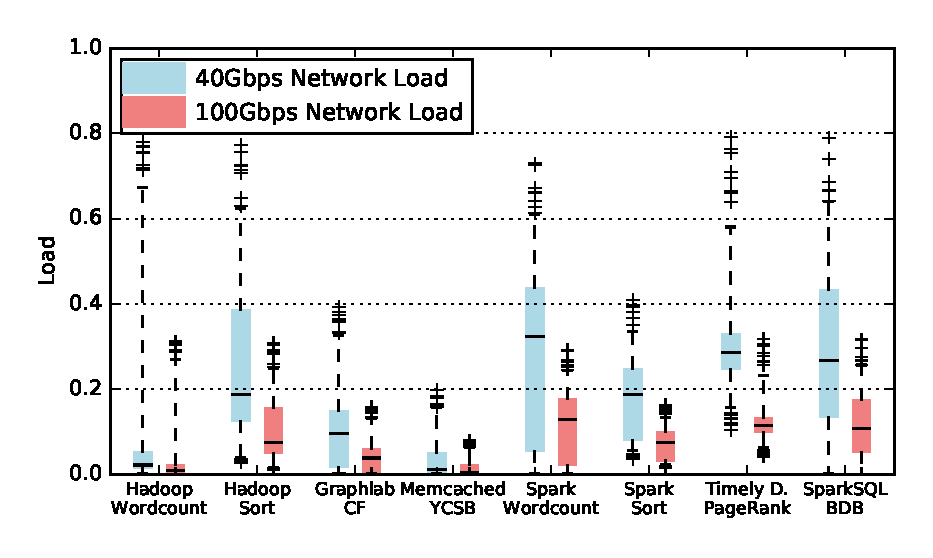
\includegraphics[width = \columnwidth]{img/load} 
  \caption{\small{Per-link load in each application. Among hosts, for each application there is significant variance in the load injected. This highlights the skewness of our traffic matrix.}}
  \label{fig:loadcdf}
\end{figure}



\paragraphb{Traffic Generation}
As mentioned above, the disaggregated datacenter we simulate includes %$144$ nodes.
9 racks. Reflecting our EC2 testbed with 5 servers, we populate each rack with  5 CPU blades, 5 memory blades and 5 storage blades.
%per cluster. The remaining 9 nodes are unused.
%Each CPU blade is associated with 12 remote memory and disk blades (i.e., the `VM' abstraction in our simulation comprises one CPU whose memory and disk address space is spread across 12 remote blades). 
To simulate rack-local clusters each rack is treated as a disaggregated cluster. 
To simulate datacenter-scale clusters, blades across the 9 racks are grouped uniformly into clusters of 15.
In the traditional datacenter topology, a single endpoint corresponds to one server blade that includes one unit each of CPU, memory \emph{and} disk. In contrast, in the disaggregated topology, a single endpoint corresponds to three units of a single resource; i.e., 3x of CPU, disk \emph{or} memory. This ensures we maintain resource parity between the traditional datacenter topology and our disaggregated one.


%given that a traditional datacenter with our topology would contain 144 each of compute, memory, and storage blades, we pack each endpoint in our simulated topology with 3 of the given resource to maintain resource parity.



Given our topology, we generate traffic for each disaggregated cluster as follows. From our workload traffic traces, we generate CDFs representing the various distributions of flow sizes and flow inter-arrival times for each source-destination pair in the cluster (note that there is no direct traffic between memory and storage blades, nor between compute blades).
%, for a total of 100 possible size and interarrival time CDF pairs 
Each endpoint in our topology is designated as a CPU, memory or disk blade and 
generates traffic by drawing from the CDFs corresponding to its resource type.
%we assign it an identity as one of our 15 disaggregated blades within its cluster and 
%draw from the appropriate CDFs to generate flows to each of the other blades in the cluster.
Since we pack resources by a factor of 3, each endpoint independently draws from its flow generation distributions three times. 
The resulting injected load can be seen in Figure~\ref{fig:loadcdf}. 
%\an{Note that with a $40$Gbps link bandwidth, load on some sources approaches 0.8}. 





\subsection{Network-level performance}
\label{ssec:nlp}

We evaluate the performance of our candidate transport protocols in terms of their  mean slowdown~\cite{pfabric}, which is computed as follows. The slowdown for a flow is computed by dividing the flow completion time achieved in simulation by the time that the flow would take to complete if it were alone in the network. The mean slowdown is then computed by averaging the slowdown over all flows.
Figure~\ref{fig:phostp} plots the mean slowdown for our five candidate protocols, using $100$Gbps links (all other parameters are as in \S\ref{ssec:ssmethod}). 

\paragraphb{Results} 
We make the following observations. 
First, looking at the mean slowdown for pFabric and pHost, we observe that they are reasonably close in performance (consistent with results shown in \cite{phost}) but that both protocols achieve higher mean slowdowns than reported 
in their original papers, both of which report close-to-optimal slowdowns with values close to 1.0~\cite{phost,pfabric}. And this is true even though the average network utilization in our \dis workload is in fact substantially lower than the utilization levels used in the simulation studies of ~\cite{pfabric, phost}. 
On closer examination, we found that the higher slowdowns with disaggregation are a consequence of the differences in our traffic workloads (both earlier studies used heavy-tailed traffic workloads based on measurement 
studies from existing datacenters). In our \dis workload, reflecting the 
application-driven nature of our workload, we observe many flow arrivals that 
appear very close in time (only observable on sub-10s of microsecond timescales), leading to high slowdowns for these flows. This effect is strongest in the case of the wordcount application which is why it suffers the highest slowdowns. 

Second, we note that while pFabric and pHost perform comparably, Fastpass fares worse; this is consistent with the findings reported in~\cite{phost}.

Finally, we  repeat the above simulations but this time simulate rack-scale 
disaggregation; i.e., a CPU blade's associated memory and disk blades are selected from 
its own rack. The results are shown in Figure~\ref{fig:phostp-rs}. We see that, with the exception of Fastpass, rack-scale disaggregation does not significantly alter the slowdown values. (Fastpass fares worse with rack-scale disaggregation because the centralized scheduler is not rack-local and hence the cost of contacting the scheduler is relatively greater.)
However, one should not conclude from this that rack-scale containment is not useful because our slowdown metric masks differences in the \emph{absolute} FCT values. Instead, slowdown is useful primarily to compare across different transport protocol designs. The impact of these absolute FCT values is captured in our next experiments.

\subsection{Application-level performance}
\label{ssec:alp}

We now use the FCTs obtained from the above simulations as the memory access times in our emulation methodology from \S\ref{sec:requirements}. We use the FCTs from pFabric as it achieves the best slowdowns over a range of test scenarios. 

We measure the degradation in application performance that results from injecting remote memory access times drawn from the FCTs that pFabric achieves with 40Gbps links and with 100Gbps links, in each case considering both datacenter-wide and rack-scale disaggregation. As in \S\ref{sec:requirements}, we measure performance degradation compared to the baseline of performance without disaggregation (i.e., injecting zero latency). 

In all cases, we find that the inclusion of queueing delay \emph{does} have a non-trivial impact on performance degradation -- typically increasing the performance degradation relative to the case of zero-queueing delay by between 2-3x. 
Figure~\ref{fig:appfabric100} plots the performance degradation for 100Gbps links: we see that degradation ranges between 1-8.5\% on average with datacenter scale disaggregation, and containment to a rack lowers the degradation to between 0.4-3.5\% on average. In topologies with 40Gbps links, we find a median performance degradation of 17\% with datacenter-scale disaggregation (figure not shown). 
This leads us to conclude that 100Gbps links are both required and sufficient to contain the performance impact of queueing delay.

\begin{figure*}
  \centering
    \subfigure[Datacenter-Scale Disaggregation]{
      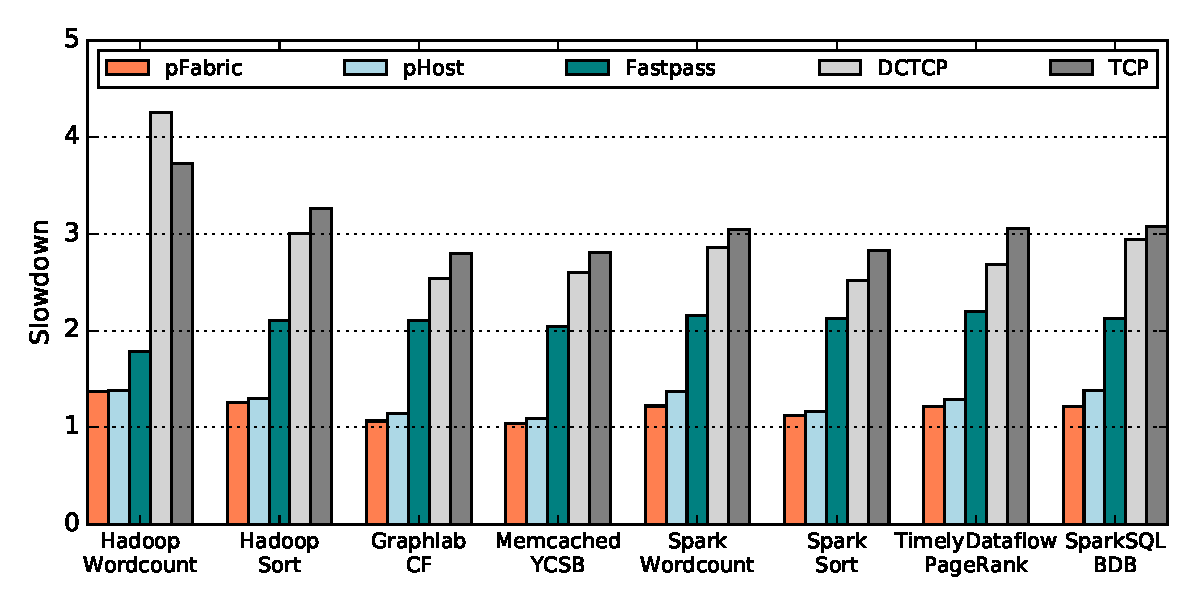
\includegraphics[width = 0.475\textwidth]{img/slowdowns/100g/allFlows_dc-scale_slowdowns} 
      \label{fig:phostp-dc}
    }
    \subfigure[Rack-Scale Disaggregation]{
      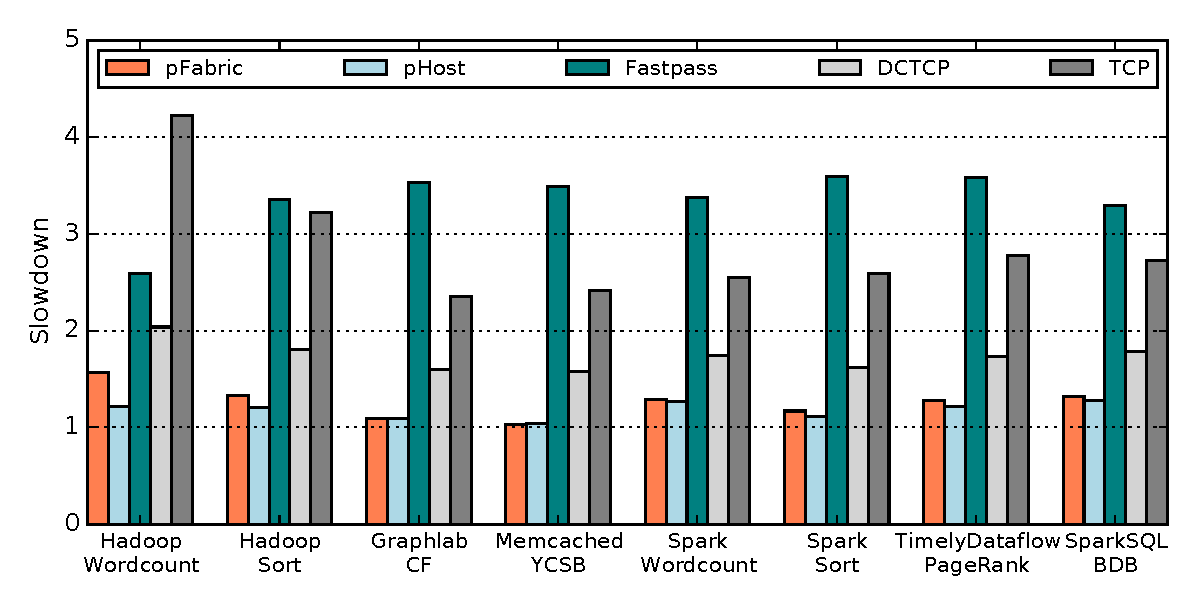
\includegraphics[width = 0.475\textwidth]{img/slowdowns/100g/allFlows_rack-scale_slowdowns} 
      \label{fig:phostp-rs}
    }
  \caption{\small{The performance of the five protocols for the case of $100$Gbps access link capacity. The results for $40$Gbps access links lead to similar conclusions. See \S\ref{ssec:nlp} for discussion on these results.}}
  \label{fig:phostp}
\end{figure*}


%
\begin{figure}
  \centering
    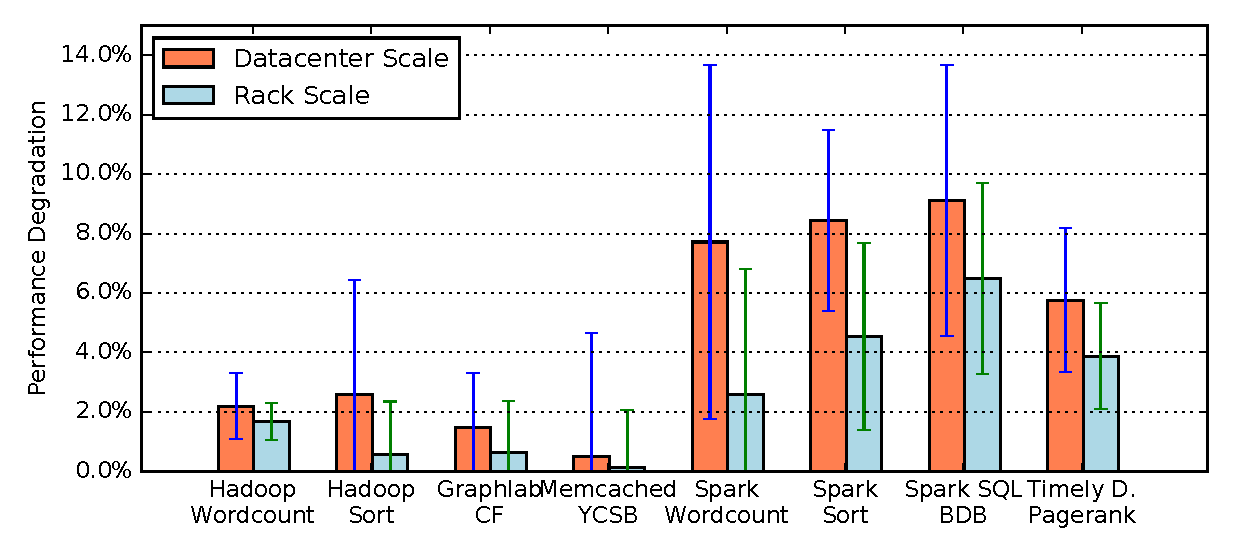
\includegraphics[width = \columnwidth]{img/slowdown.eps} 
  \caption{\small{Application layer slowdown for each of the four applications at rack-scale and datacenter scale after injecting pFabric's FCT with 100Gbps link. }}
  \label{fig:appfabric100}
\end{figure}
%



\subsection{Low latency remote memory}
\rc{
As we have established in the previously section, a DDC requires 100Gbps bandwidth and 3-5us end-to-end latency. 
Current datacenter network usually has 20us network latency, and by our analysis, 5-7us of end-to-end latency is within reach. 
If we enable RDMA inside the datacenter, which takes aways the overhead at OS layer, we can get latency as low as 3-5us. 
We validate this by building a kernel space RDMA block device driver, and use this block device driver as the swap device.
With the RDMA block device driver, the local machine can swap to remote memory instead of swapping to disk.

We implement the block device driver on a machine with Mellanox  4xFDR Infiniband card.
To maintain high throughput, we first use a batch implementation that batches block requests and sends all of them together to the RDMA NIC.
The driver waits for all the request to come back and notify the upper layer.
We test the block device throughput using \textit{dd} with direct IO, and measure the request latency by instrumenting the driver code.
The block device throughput is only 0.8GB/s and the latency is around 4-16us.
We observed that many block requests are actually contiguous in address, so we merge these request in to one large request. 
With request merging, the throughput becomes 2.6GB/s, which is ~3x better than the batch version. 
The performance of the block device driver can be further improved by issuing RDMA requests asynchronously.
We create a data structure to keep track of all the out going requests and notify the upper layer immediately for each completed request.
This improves the throughput to 3.3GB/s which is as high as a local RamFS, and reduces the request latency to 3-4us (Table \ref{tab:rdma_latency}).

\begin{table}[t]
    \centering
    \small
    \begin{tabular}{ccccc}
    \textbf{Min}	& \textbf{Avg}	& \textbf{Median} & \textbf{99.5 Pcntl}	& \textbf{Max}\\
    \hline
    3394 &	3492&	3438&	4549&	12254\\\hline
    \end{tabular}
    \caption{RDMA block device request latency(ns)}
    \label{tab:rdma_latency}
\end{table}

In current non-NUMA architecture, Linux Kernel only launches one \textit{kswapd} to swap out least recently used pages. 
This could be a bottleneck for apps that heavily use remote memory.
We enable the NUMA\_EMU feature in Linux kernel, which partitions the memory into several regions, and each memory region gets its own \textit{kswapd}. 
This improves the throughput of swapping out memory pages.


The RDMA block device driver provides us a simple and efficient way utilize remote memory. 
We setup the block device as swap space and run the \rc{5} applications evaluated in \S \ref{sec:requirements} with lower latency requirements.
\rc{waiting for joao's results}

}
